\begin{sectionbox}[Why do we need torch compile?]\nospacing
        Efficient computation graphs are important for modern deep learning applications.
        Dynamic graph computation\cref{defn:dynamic_graph_computation} for eager mode\cref{defn:eager_mode} frameworks used to work as fast as compiled graph frameworks.
        \begin{figure}[H]
            \centering
            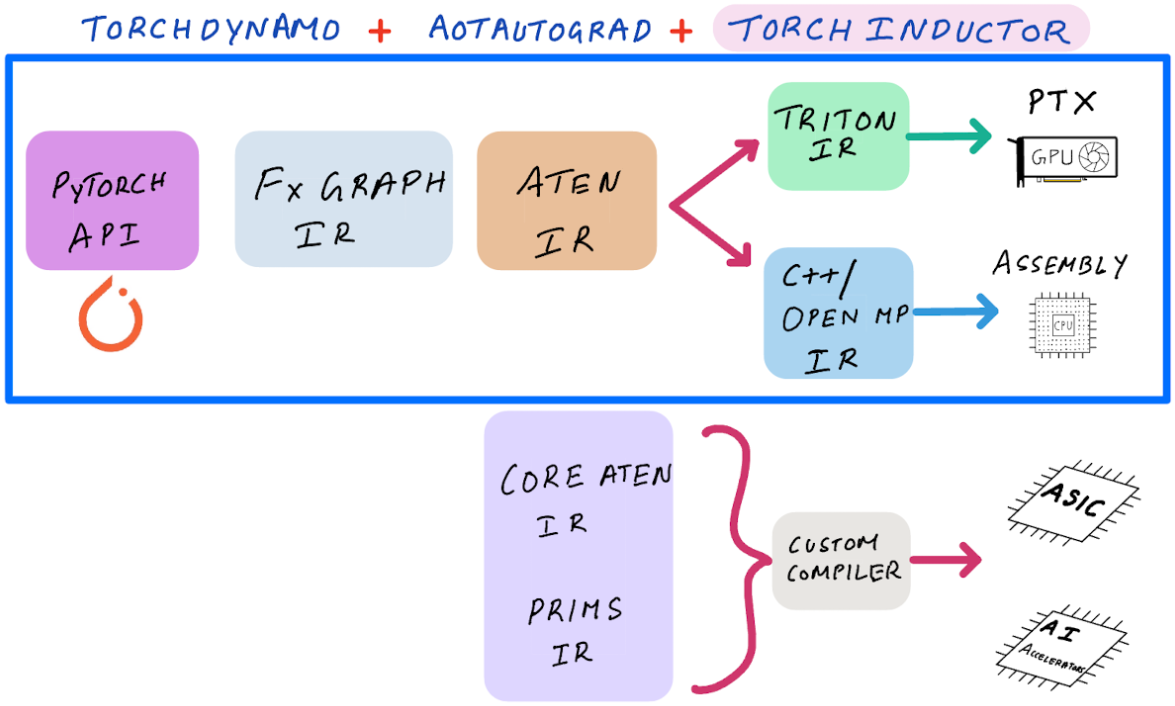
\includegraphics[width=1.0\textwidth]{pytorch_submodule/src/the_framework/graph_acquisition/figures/overview.png}
        \end{figure}
        This used to be true as long as batch sizes are small and operations are simple.
        I.e. the execution of the \textit{host} python code (+graph acquisition) used to be faster than the execution of the kernels queuing on the GPU.
        However modern accelerators are getting faster, operations getting complexer and batch size are getting bigger such that graph acquisition on the host becomes the bottleneck.
\end{sectionbox}

%%% Local Variables:
%%% mode: latex
%%% TeX-command-extra-options: "-shell-escape"
%%% TeX-master: "../../../../formulary"
%%% End:
